\documentclass{beamer}

\usepackage{gensymb}
\usepackage[utf8]{inputenc}
\DeclareUnicodeCharacter{00A0}{ }%Permet d'éviter certains conflits de caractères invisibles
\usepackage{amssymb}            % Principaux symboles
%\usepackage{fontspec}
%\usepackage{xunicode}
%\usepackage{xltxtra}
\usepackage[frenchb]{babel}
%\defaultfontfeatures{Scale=MatchLowercase}
%\setmainfont[Mapping=tex-text,Ligatures={Common, Historical}]{Linux Libertine O}
%\setsansfont[Mapping=tex-text]{Linux Biolinum O}
%\setmonofont[Scale=0.75]{DejaVu Sans Mono}

%% Packages pour le texte
%\usepackage[misc,geometry]{ifsym}	% Police numéros battons
\usepackage{pifont}		% Police \ding
\usepackage{eurosym}		% Symbole de l'euro
\usepackage{soul}		% Souligner
\usepackage{enumerate}		% Listes
\usepackage{verbatim}		% Codes source
\usepackage{moreverb}		%	et listings
\usepackage{textcomp}
\usepackage{multicol}

%% Packages pour les tableaux
\usepackage{array}		% Outils supplémentaires
\usepackage{multirow}		% Colonnes multiples
\usepackage{tabularx}		% Largeur totale donnée
\usepackage{longtable}		% Sur plusieurs pages

%% Les packages pour les dessins
\usepackage{graphicx}		% Insertion de figures
%\usepackage{picins}		% Dans un paragraphe
\usepackage{epic}		% Capacités graphiques
\usepackage{eepic}		% 	étendues
\usepackage{afterpage}		% Voir page 69
\usepackage{rotating}		% Tourner du texte
\usepackage{caption}		% Légendes
% \addto\captionsfrench{\def\figurename{}}

%% Packages pour les maths
\usepackage{amsmath}		% Commandes essentielles
\usepackage{amssymb}		% Principaux symboles
\usepackage{mathrsfs}		% Police calligraphique
\usepackage{theorem}		% Théorèmes
%\usepackage{tikz}		% Courbes
\usepackage{esvect}            % Vecteurs
%\usetikzlibrary{shapes,arrows,shadows}
\usepackage{pgf}
%\usetikzlibrary{arrows}
% Packages pour la physique
%\usepackage{sistyle}		% Unités
\usepackage[version=3]{mhchem}	% Formules chimiques
\usepackage{etex}
%\usepackage{m-pictex,m-ch-en}

%\usepackage{media9}
\usepackage{multimedia}		% Vidéos dans la présentation
%\usepackage{movie15}

%Ajout d'images de fond:
\usepackage{eso-pic}
\usepackage{wallpaper}

\usepackage{ccicons}		% Licence creativecommons

%\SIdecimalsign{,}


\AtBeginSection[]
{
  \begin{frame}
    \frametitle{Sommaire}
    \begin{multicols}{2}
      {\small
				\setcounter{tocdepth}{2}
        \tableofcontents[currentsection, hideothersubsections]}
    \end{multicols}
  \end{frame}
}

\usetheme{Warsaw}

\usepackage{listings}
\usepackage[babel=true]{csquotes}
\lstset{language=Python, tabsize=2, breaklines=true, showstringspaces=false}

\definecolor{RedT}{rgb}{1, .7, .7}
\definecolor{GreenT}{rgb}{.7, 1, .7}
\definecolor{OrangeT}{rgb}{1, 1, .7}

\useoutertheme{infolines}
\setbeamersize{text margin left=1cm,text margin right=1cm}

\title{Rapport de projet de SI}
\subtitle{Tropodrone}
\author{Gueydan Noé, Manceau Thibaut, Gros Alexis, Porteries Tristan}

\begin{document}

\begin{frame}
  \titlepage
\end{frame}

\begin{frame}
    \frametitle{Sommaire}
    \begin{multicols}{2}
      {
		\setcounter{tocdepth}{1}
        \tableofcontents
      }
    \end{multicols}
\end{frame}

\section{Courte présentation}

\subsection{But du projet}
\begin{frame}{But du projet}
 Créer une structure composée de ballons contenant un gaz plus léger que l’air qui soutient une partie ou la totalité du poids d'un drone.
\end{frame}


\subsection{Objectifs}
\begin{frame}{Objectifs}
 Augmenter l’autonomie, la sécurité et les possibilités d’un drone de petite taille
\end{frame}


\subsection{Contraintes imposées au projet}
\begin{frame}{Contraintes imposées au projet}
  \begin{itemize}
    \item être simple d’utilisation, garder la manœuvrabilité du drone au possible, voler le plus longtemps possible~;
    \item consommer le moins d’énergie possible, ne pas présenter de danger pour le public et économiser le gaz et les matériaux de fabrication~;
    \item le modèle du drone imposé~;
    \item rayon d’action de minimum 15 mètres~;
    \item ballon de type dirigeable.
  \end{itemize}
\end{frame}

\subsection{Contraintes légales supplémentaires}
\begin{frame}{Contraintes légales supplémentaires}
  \begin{itemize}
    \item 1~: Le drone \\
	    catégorie A~: limitations non contraignantes~;
    \item 2~: Le ballon \\
	    catégorie « Léger » \\
	    la ficelle supportant la charge doit casser au dessus de 23 kg.
 \end{itemize}
\end{frame}


\section{Drone}

\subsection{Modèle}

\begin{frame}
  \begin{multicols}{2}
    Drone XCSOURCE~: \\
    \begin{itemize}
      \item 290 mm diagonale~;
      \item 190 mm longueur~;
      \item 70 mm hauteur~;
      \item moteur EMAX MT2204 2300KV Brushless Motor~;
      \item Accu Lipo Gens Ace 2200Mah 11.1V 25C 3S~;
      \item 450 g.
    \end{itemize}
    \newpage
    \begin{center}
      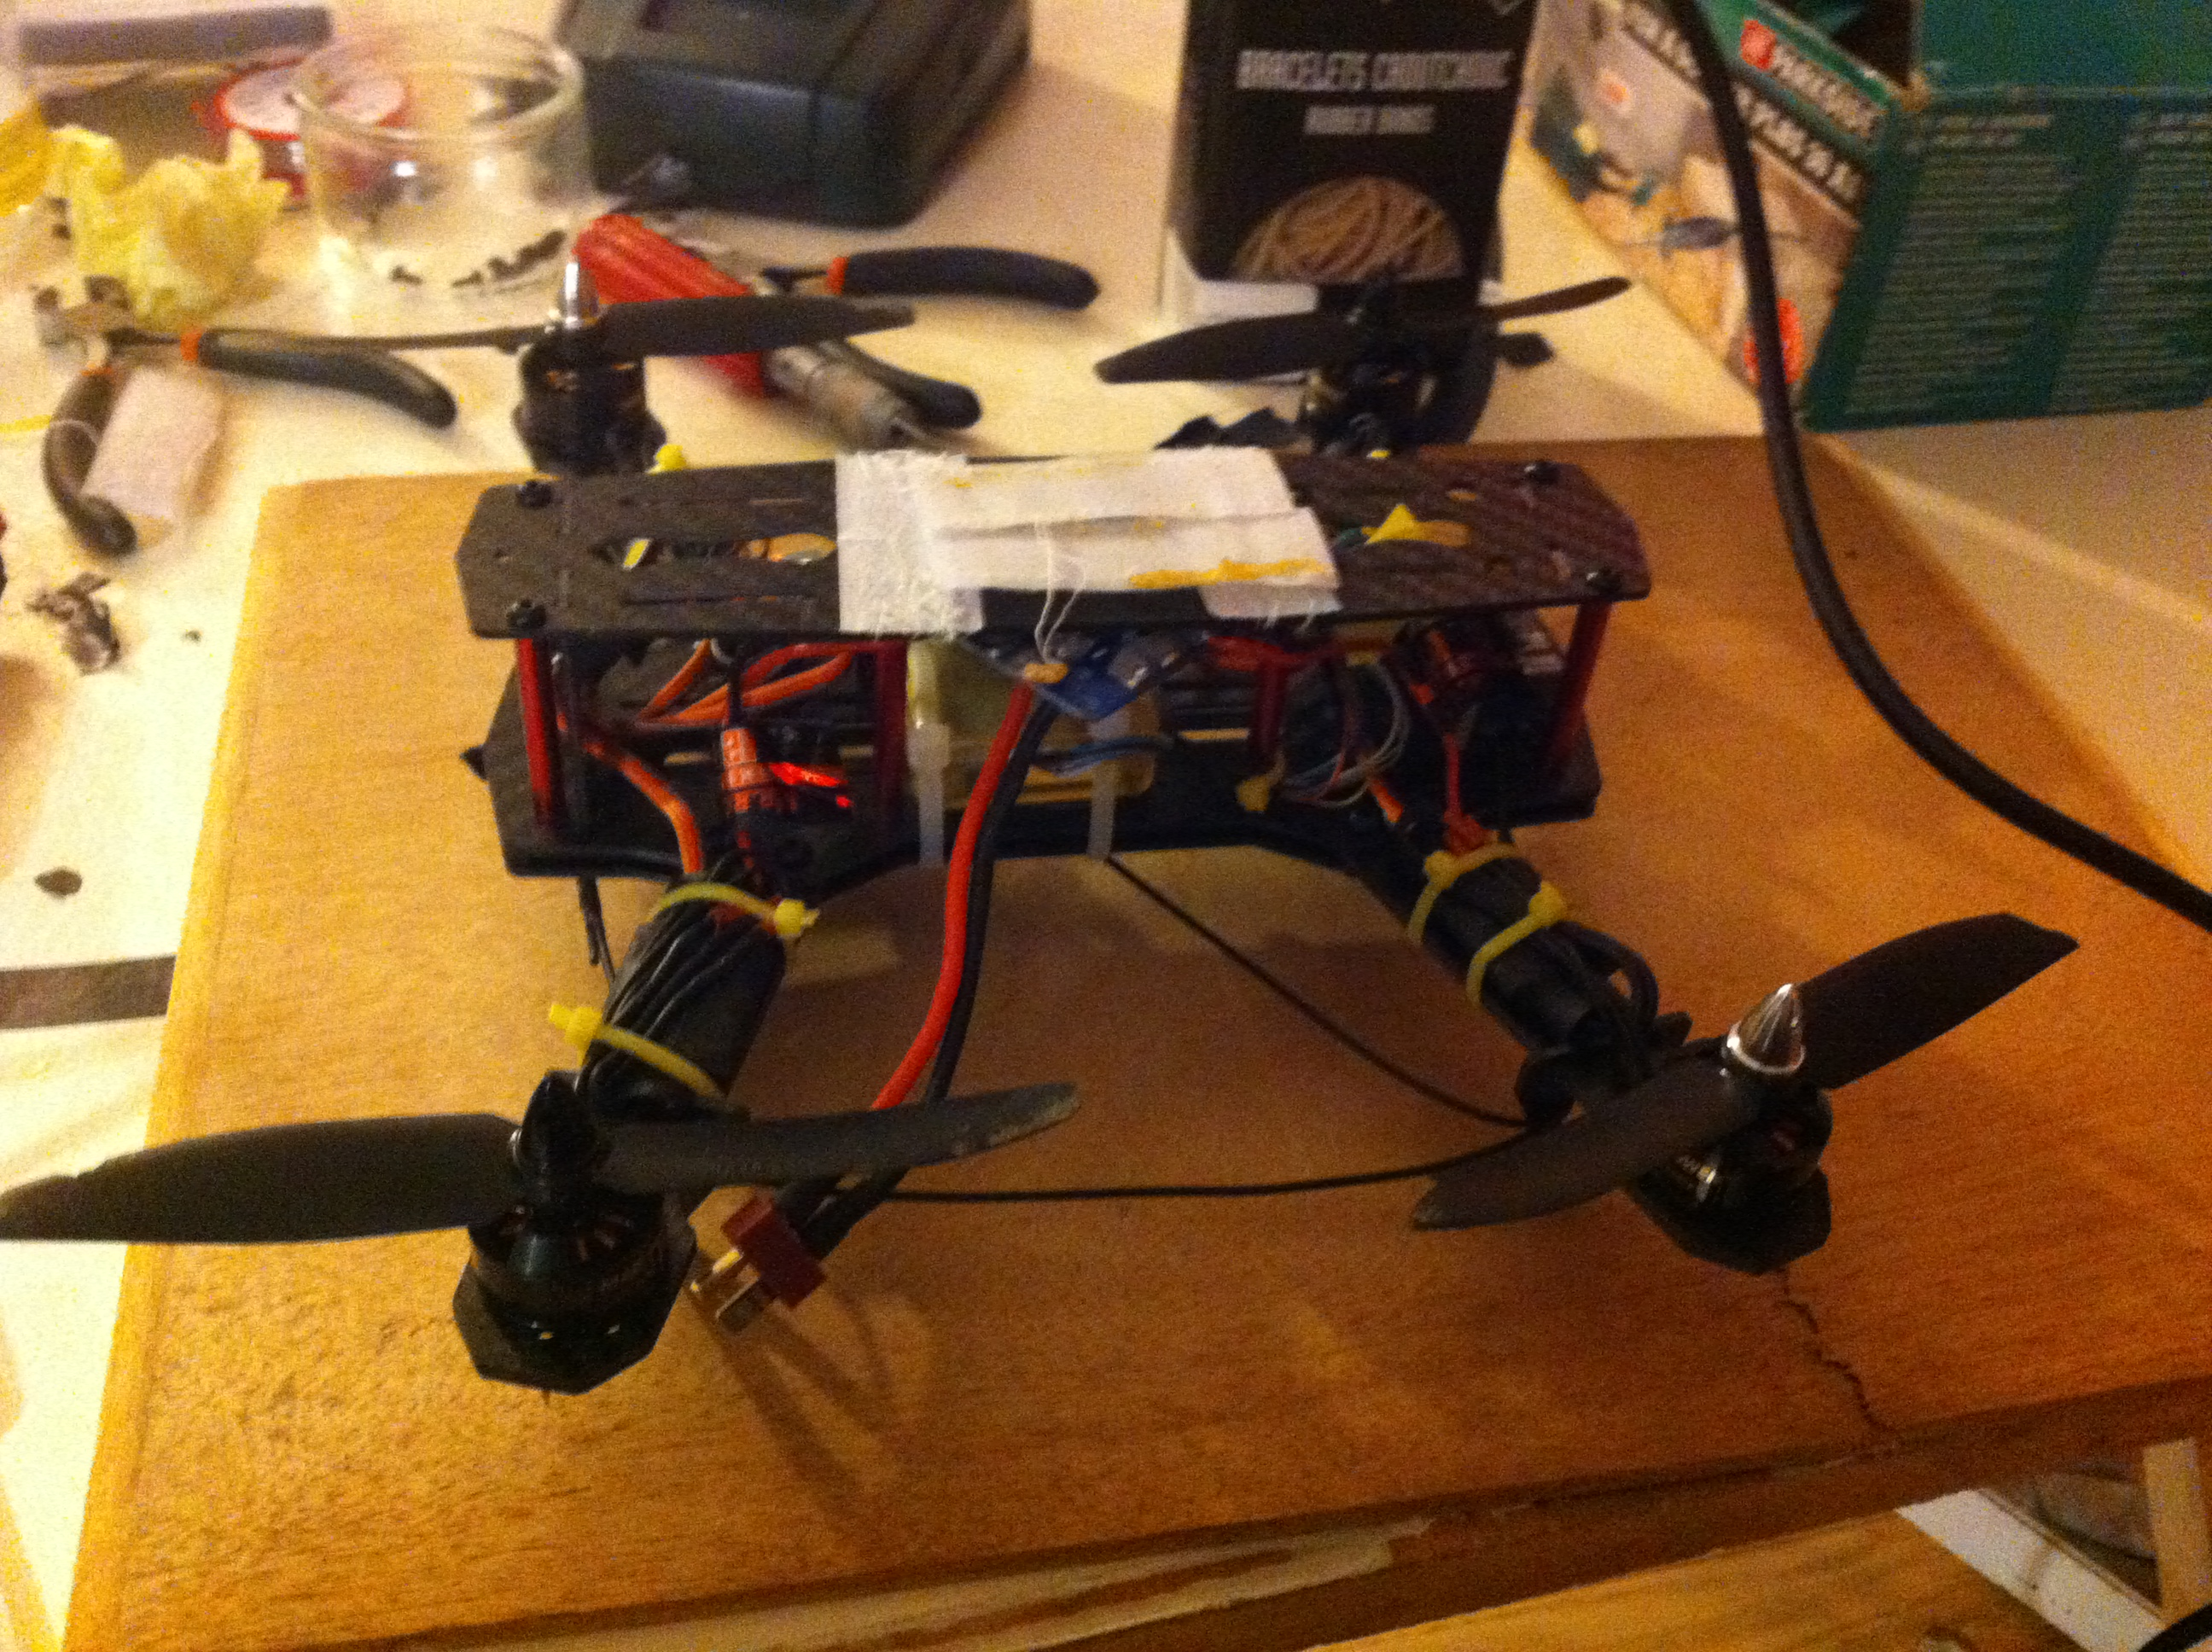
\includegraphics[width=6cm]{../Images/drone.JPG}
    \end{center}
    \captionof{figure}{Drone XCSOURCE.}
  \end{multicols}
\end{frame}




\section{Aérodynamisme}

\begin{frame}{Objectif}
 But : que le drone soit le moins sensible à l'air possible. \\
 \textbf{Garder la manœuvrabilité du drone au possible}
\end{frame}

\subsection{Équation de traînée}
\begin{frame}{Équation de traînée}
  \begin{center}
		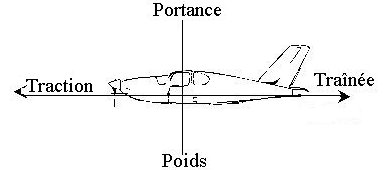
\includegraphics[width=5cm]{../Images/portance.jpg}
	\end{center}
 Force de traînée matérialisée par l'équation \\
 \begin{center}
  \boxed{\displaystyle{\frac12 \times \rho \times S \times Cx \times V^2}}
 \end{center}
 Avec~:
 \begin{itemize}
  \item $\rho$ la masse volumique du fluide dans lequel a lieu le déplacement en $kg.m^{-3}$~;
  \item S la surface~;
  \item Cx le coefficient de traînée~;
  \item V la vitesse relative du mobile par rapport au fluide en $m.s^{-1}$.
 \end{itemize}
\end{frame}

\subsection{Problèmes et solutions techniques}
\begin{frame}{Problème des ballons}
  \begin{itemize}
	\item 3 ballons de 0.25 m³ : surface à réduire
  \item Cx différent selon position des ballons face au flux d'air
\end{itemize}
\end{frame}

\begin{frame}{La forme en triangle}
	Permet de créer un couloir dans lequel le vent s'engouffre.
  \begin{center}
		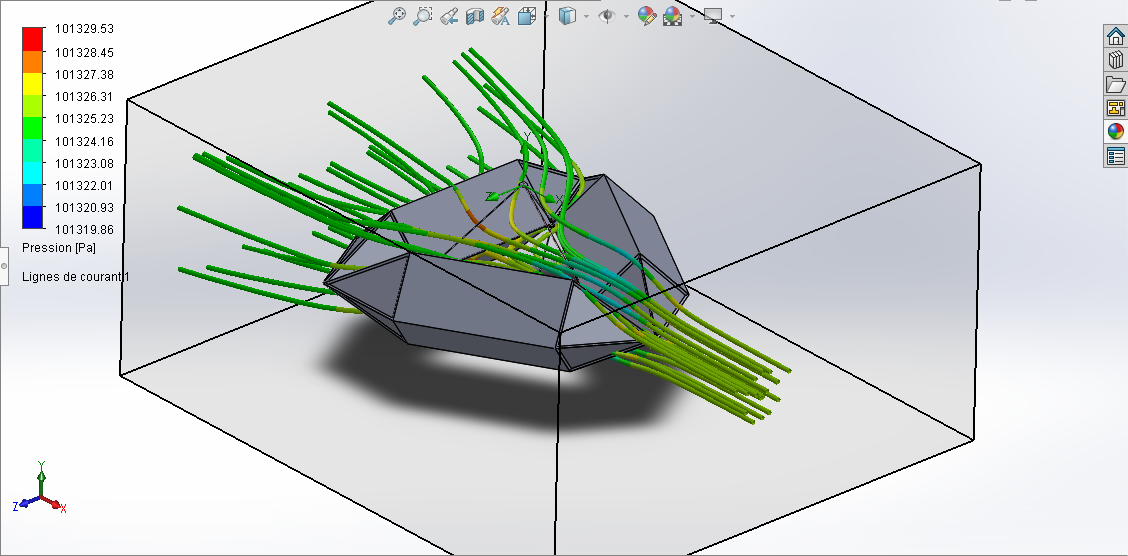
\includegraphics[width=10cm]{../Images/Capture.PNG}
	\end{center}
\end{frame}

\begin{frame}{Gouvernail}
	Le gouvernail permet d'orienter les ballons en fonction de la direction du drone.\\
  Assimilable aux conformations d'une molécule~:
  \begin{center}
		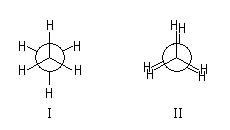
\includegraphics[width=10cm]{../Images/conformations.png}
	\end{center}
\end{frame}

\subsection{Résolution de l'équation}
\begin{frame}{Résolution pour une sphère}
\begin{center}
 \boxed{\displaystyle{Re = \frac{V \times L}{\nu}}}
\end{center}
Avec~:
\begin{itemize}
 \item $Re$ la masse volumique du fluide dans lequel a lieu le déplacement en $kg.m^{-3}$~;
 \item V la vitesse relative du mobile par rapport au fluide en $m.s^{-1}$;
 \item L la dimension caractéristique (ici le diamètre de la sphère)~;
 \item $\nu$ la viscosité cinématique du fluide~;
\end{itemize}
\end{frame}

\begin{frame}{Résolution pour une sphère - Algorithme}
  \begin{center}
    \lstset{language={Python}}
    \lstinputlisting{../Aerodynamisme/Programmes/calculTraineeReduit.py}
  \end{center}
\end{frame}

\begin{frame}{Résolution pour une sphère - Algorithme}
  \begin{center}
    \lstset{language={Python}}
    \lstinputlisting{../Aerodynamisme/Programmes/calculTraineeReduit2.py}
  \end{center}
\end{frame}

\begin{frame}{Résolution sous SW - 1}
  \begin{center}
    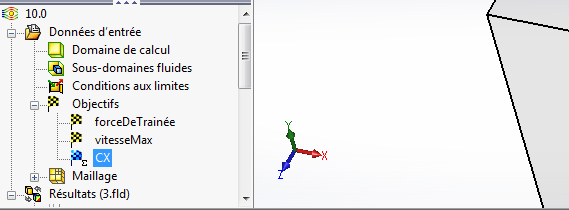
\includegraphics[width=10cm]{../Images/objectifsSW.png}
    \captionof{figure}{Objectif de calcul pour déterminer F.}
  \end{center}
\end{frame}

\begin{frame}{Résolution sous SW - 2}
  \begin{center}
    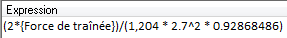
\includegraphics[width=5cm]{../Images/expressionCX.png}
    \captionof{figure}{Objectif de calcul pour déterminer Cx.}
  \end{center}
\end{frame}

\begin{frame}{Résolution sous SW - 3}
	\begin{center}
		\begin{tabular}{c}
      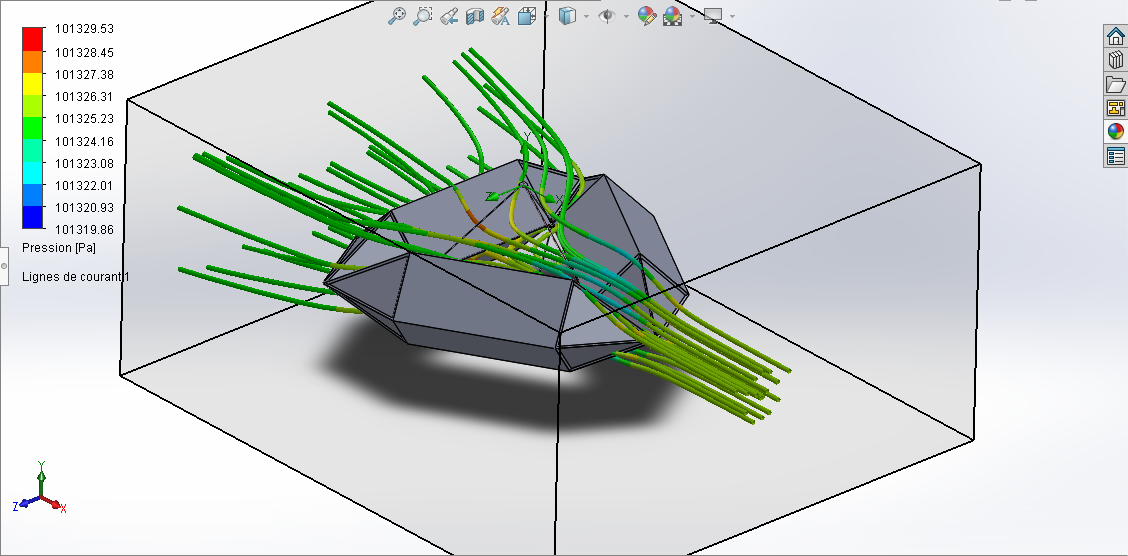
\includegraphics[width=10cm]{../Images/Capture.PNG} \\
			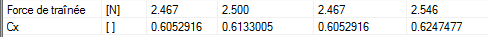
\includegraphics[width=8cm]{../Images/resultatsSimulationSW.png}
		\end{tabular}
	\end{center}
\end{frame}

\begin{frame}{Conclusion - Données de SW}
	\begin{center}
    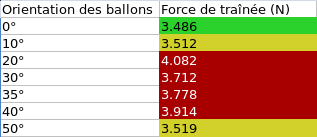
\includegraphics[width=10cm]{../Images/resultatsSW.png} \\
	\end{center}
\end{frame}

\begin{frame}{Conclusion}
  Le gouvernail présente un réel intérêt.\\
  Le drone peut lutter jusqu'à une vitesse de 20 km.h-¹
\end{frame}

\begin{frame}{Conclusion}
  \begin{center}
  FIN
  \end{center}
\end{frame}

\end{document}
